%File: formatting-instructions-latex-2025.tex
%release 2025.0
\documentclass[letterpaper]{article} % DO NOT CHANGE THIS
\usepackage{aaai25}  % DO NOT CHANGE THIS
\usepackage{times}  % DO NOT CHANGE THIS
\usepackage{helvet}  % DO NOT CHANGE THIS
\usepackage{courier}  % DO NOT CHANGE THIS
\usepackage[hyphens]{url}  % DO NOT CHANGE THIS
\usepackage{graphicx} % DO NOT CHANGE THIS
\urlstyle{rm} % DO NOT CHANGE THIS
\def\UrlFont{\rm}  % DO NOT CHANGE THIS
\usepackage{natbib}  % DO NOT CHANGE THIS AND DO NOT ADD ANY OPTIONS TO IT
\usepackage{caption} % DO NOT CHANGE THIS AND DO NOT ADD ANY OPTIONS TO IT
\frenchspacing  % DO NOT CHANGE THIS
\setlength{\pdfpagewidth}{8.5in}  % DO NOT CHANGE THIS
\setlength{\pdfpageheight}{11in}  % DO NOT CHANGE THIS
%
% These are recommended to typeset algorithms but not required. See the subsubsection on algorithms. Remove them if you don't have algorithms in your paper.
\usepackage{algorithm}
\usepackage{algorithmic}
\usepackage{booktabs}
\usepackage{multirow}
\usepackage{xcolor}

%
% These are are recommended to typeset listings but not required. See the subsubsection on listing. Remove this block if you don't have listings in your paper.
\usepackage{newfloat}
\usepackage{listings}
\DeclareCaptionStyle{ruled}{labelfont=normalfont,labelsep=colon,strut=off} % DO NOT CHANGE THIS
\lstset{%
	basicstyle={\footnotesize\ttfamily},% footnotesize acceptable for monospace
	numbers=left,numberstyle=\footnotesize,xleftmargin=2em,% show line numbers, remove this entire line if you don't want the numbers.
	aboveskip=0pt,belowskip=0pt,%
	showstringspaces=false,tabsize=2,breaklines=true}
\floatstyle{ruled}
\newfloat{listing}{tb}{lst}{}
\floatname{listing}{Listing}
%
% Keep the \pdfinfo as shown here. There's no need
% for you to add the /Title and /Author tags.
\pdfinfo{
/TemplateVersion (2025.1)
}

\usepackage{amsmath, amssymb}

% DISALLOWED PACKAGES
% \usepackage{authblk} -- This package is specifically forbidden
% \usepackage{balance} -- This package is specifically forbidden
% \usepackage{color (if used in text)
% \usepackage{CJK} -- This package is specifically forbidden
% \usepackage{float} -- This package is specifically forbidden
% \usepackage{flushend} -- This package is specifically forbidden
% \usepackage{fontenc} -- This package is specifically forbidden
% \usepackage{fullpage} -- This package is specifically forbidden
% \usepackage{geometry} -- This package is specifically forbidden
% \usepackage{grffile} -- This package is specifically forbidden
% \usepackage{hyperref} -- This package is specifically forbidden
% \usepackage{navigator} -- This package is specifically forbidden
% (or any other package that embeds links such as navigator or hyperref)
% \indentfirst} -- This package is specifically forbidden
% \layout} -- This package is specifically forbidden
% \multicol} -- This package is specifically forbidden
% \nameref} -- This package is specifically forbidden
% \usepackage{savetrees} -- This package is specifically forbidden
% \usepackage{setspace} -- This package is specifically forbidden
% \usepackage{stfloats} -- This package is specifically forbidden
% \usepackage{tabu} -- This package is specifically forbidden
% \usepackage{titlesec} -- This package is specifically forbidden
% \usepackage{tocbibind} -- This package is specifically forbidden
% \usepackage{ulem} -- This package is specifically forbidden
% \usepackage{wrapfig} -- This package is specifically forbidden
% DISALLOWED COMMANDS
% \nocopyright -- Your paper will not be published if you use this command
% \addtolength -- This command may not be used
% \balance -- This command may not be used
% \baselinestretch -- Your paper will not be published if you use this command
% \clearpage -- No page breaks of any kind may be used for the final version of your paper
% \columnsep -- This command may not be used
% \newpage -- No page breaks of any kind may be used for the final version of your paper
% \pagebreak -- No page breaks of any kind may be used for the final version of your paperr
% \pagestyle -- This command may not be used
% \tiny -- This is not an acceptable font size.
% \vspace{- -- No negative value may be used in proximity of a caption, figure, table, section, subsection, subsubsection, or reference
% \vskip{- -- No negative value may be used to alter spacing above or below a caption, figure, table, section, subsection, subsubsection, or reference

\setcounter{secnumdepth}{0} %May be changed to 1 or 2 if section numbers are desired.

% The file aaai25.sty is the style file for AAAI Press
% proceedings, working notes, and technical reports.
%

% Title

% Your title must be in mixed case, not sentence case.
% That means all verbs (including short verbs like be, is, using,and go),
% nouns, adverbs, adjectives should be capitalized, including both words in hyphenated terms, while
% articles, conjunctions, and prepositions are lower case unless they
% directly follow a colon or long dash
\title{Hierarchical DeepPruner: A Novel Framework for Search Space Reduction}
\author{
    %Authors
    % All authors must be in the same font size and format.
    Ankur Nath, Alan Kuhnle
}
\affiliations{
    %Afiliations
    Department of Computer Science \& Engineering, Texas A\&M University\\
    anath@tamu.edu, kuhnle@tamu.edu
}

%Example, Single Author, ->> remove \iffalse,\fi and place them surrounding AAAI title to use it
\iffalse
\title{My Publication Title --- Single Author}
\author {
    Author Name
}
\affiliations{
    Affiliation\\
    Affiliation Line 2\\
    name@example.com
}
\fi

\iffalse
%Example, Multiple Authors, ->> remove \iffalse,\fi and place them surrounding AAAI title to use it
\title{My Publication Title --- Multiple Authors}
\author {
    % Authors
    First Author Name\textsuperscript{\rm 1,\rm 2},
    Second Author Name\textsuperscript{\rm 2},
    Third Author Name\textsuperscript{\rm 1}
}
\affiliations {
    % Affiliations
    \textsuperscript{\rm 1}Affiliation 1\\
    \textsuperscript{\rm 2}Affiliation 2\\
    firstAuthor@affiliation1.com, secondAuthor@affilation2.com, thirdAuthor@affiliation1.com
}
\fi




\begin{document}

\maketitle

\begin{abstract}
Combinatorial optimization (CO) problems on graphs arise in various applications across diverse domains. Many of these problems are NP-hard, and heuristics have been developed to provide near-optimal solutions. In the big data era, the high dimensionality of these problems poses significant challenges for existing heuristic methods, which struggle to scale efficiently. In this paper, we propose \textbf{Hierarchical DeepPruner}, an adaptive framework that employs a two-stage approach to efficiently prune the search space of CO problems on graphs. Compared to state-of-the-art pruning heuristics, our algorithm offers two key advantages: (\romannumeral 1) it does not require extensive feature engineering or domain-specific knowledge, and (\romannumeral 2) it outperforms all previous methods while consistently pruning over 95\% of the ground set, resulting in up to several of tenfold speedups—typically with minimal impact on solution quality. Additionally, our algorithm can successfully reduce the search space of instances even if they lie outside the training distribution, resulting in small optimality gaps across multiple budgets. 
\end{abstract}

% Uncomment the following to link to your code, datasets, an extended version or similar.
%
% \begin{links}
%     \link{Code}{https://aaai.org/example/code}
%     \link{Datasets}{https://aaai.org/example/datasets}
%     \link{Extended version}{https://aaai.org/example/extended-version}
% \end{links}


\section{Introduction}

Consider the problem of selecting influential individuals in a social network to receive free product samples, aiming to trigger a cascade of product adoptions through word of mouth. This problem is computationally challenging, as finding an exact solution is NP-hard \cite{kempe2003maximizing}. While heuristics can offer approximate solutions for this problem, they often struggle to scale due to the sheer size of typical social networks. Moreover, many individuals are poor candidates for selection, such as those with limited social connections. Instead of considering the entire population, we can focus on a smaller subset of highly influential individuals who are more likely to reach a broad and diverse audience, thereby maximizing the reach of the cascade. This allows us to efficiently apply existing heuristics or exact methods within the smaller subset without compromising solution quality.

This idea naturally extends to any combinatorial optimization problem, where the objective is to find the maxima or minima of a function over a large discrete configuration space. Finding the optimal solution to a CO problem requires an exhaustive search of the solution space; with many canonical CO problems being NP-hard \cite{karp2009reducibility}, this usually means that they are unsolvable in practice. However, exactly optimal solutions are often not required, and many heuristic approaches have been developed to obtain near-optimal solutions in polynomial time \cite{nemhauser1978analysis,kempe2003maximizing,tang2015influence}.  More frequently, the practical application of these algorithms involves very large graphs. This significantly increases the run time of the heuristics. In this work, we explore how reducing the search space—by identifying and focusing on a promising subset of candidates—can improve the scalability of heuristics for CO problems under size constraint. Formally, we have the following problem definition.


\paragraph{Problem Definition (Pruning).} We are given a combinatorial optimization problem consisting of a ground set \(\mathcal{U}\) and an exact method \(\mathcal{OPT}\) for the problem. An optimal solution is defined as a subset of the ground set \(X^\star = \mathcal{OPT} (\mathcal{U}) \) that maximizes the objective function \(f(\cdot)\) while satisfying the size constraint \(|X| \leq B\), i.e


\[X^\star  = \text{arg max}_{X \subset  \mathcal{U},|X|\leq B} f(X)\]

The problem we aim to address is finding a significantly smaller ground set \(\mathcal{U}'\), such that \(|\mathcal{U}'| \ll |\mathcal{U}|\), while ideally preserving the objective value, i.e.,  
\[
\frac{f(\mathcal{OPT}(\mathcal{U}'))}{f(\mathcal{OPT}(\mathcal{U}))} = 1. \]  


Recently, there has been a growing trend of applying machine learning techniques for pruning \cite{lauri2019fine, grassia2019learning, sun2021generalization, ireland2022lense, tian2024combhelper}. While these machine learning models have shown effectiveness for specific CO problems, they often require domain-specific knowledge and substantial feature engineering to achieve satisfactory performance. Thus, in this work, we are motivated by the following question:

\begin{center}
  \textit{Is it possible to develop a pruning algorithm that does not rely on domain-specific knowledge or feature engineering, yet remains practical and competitive with existing heuristics?}
\end{center}

\begin{figure*}[t]
    \centering
    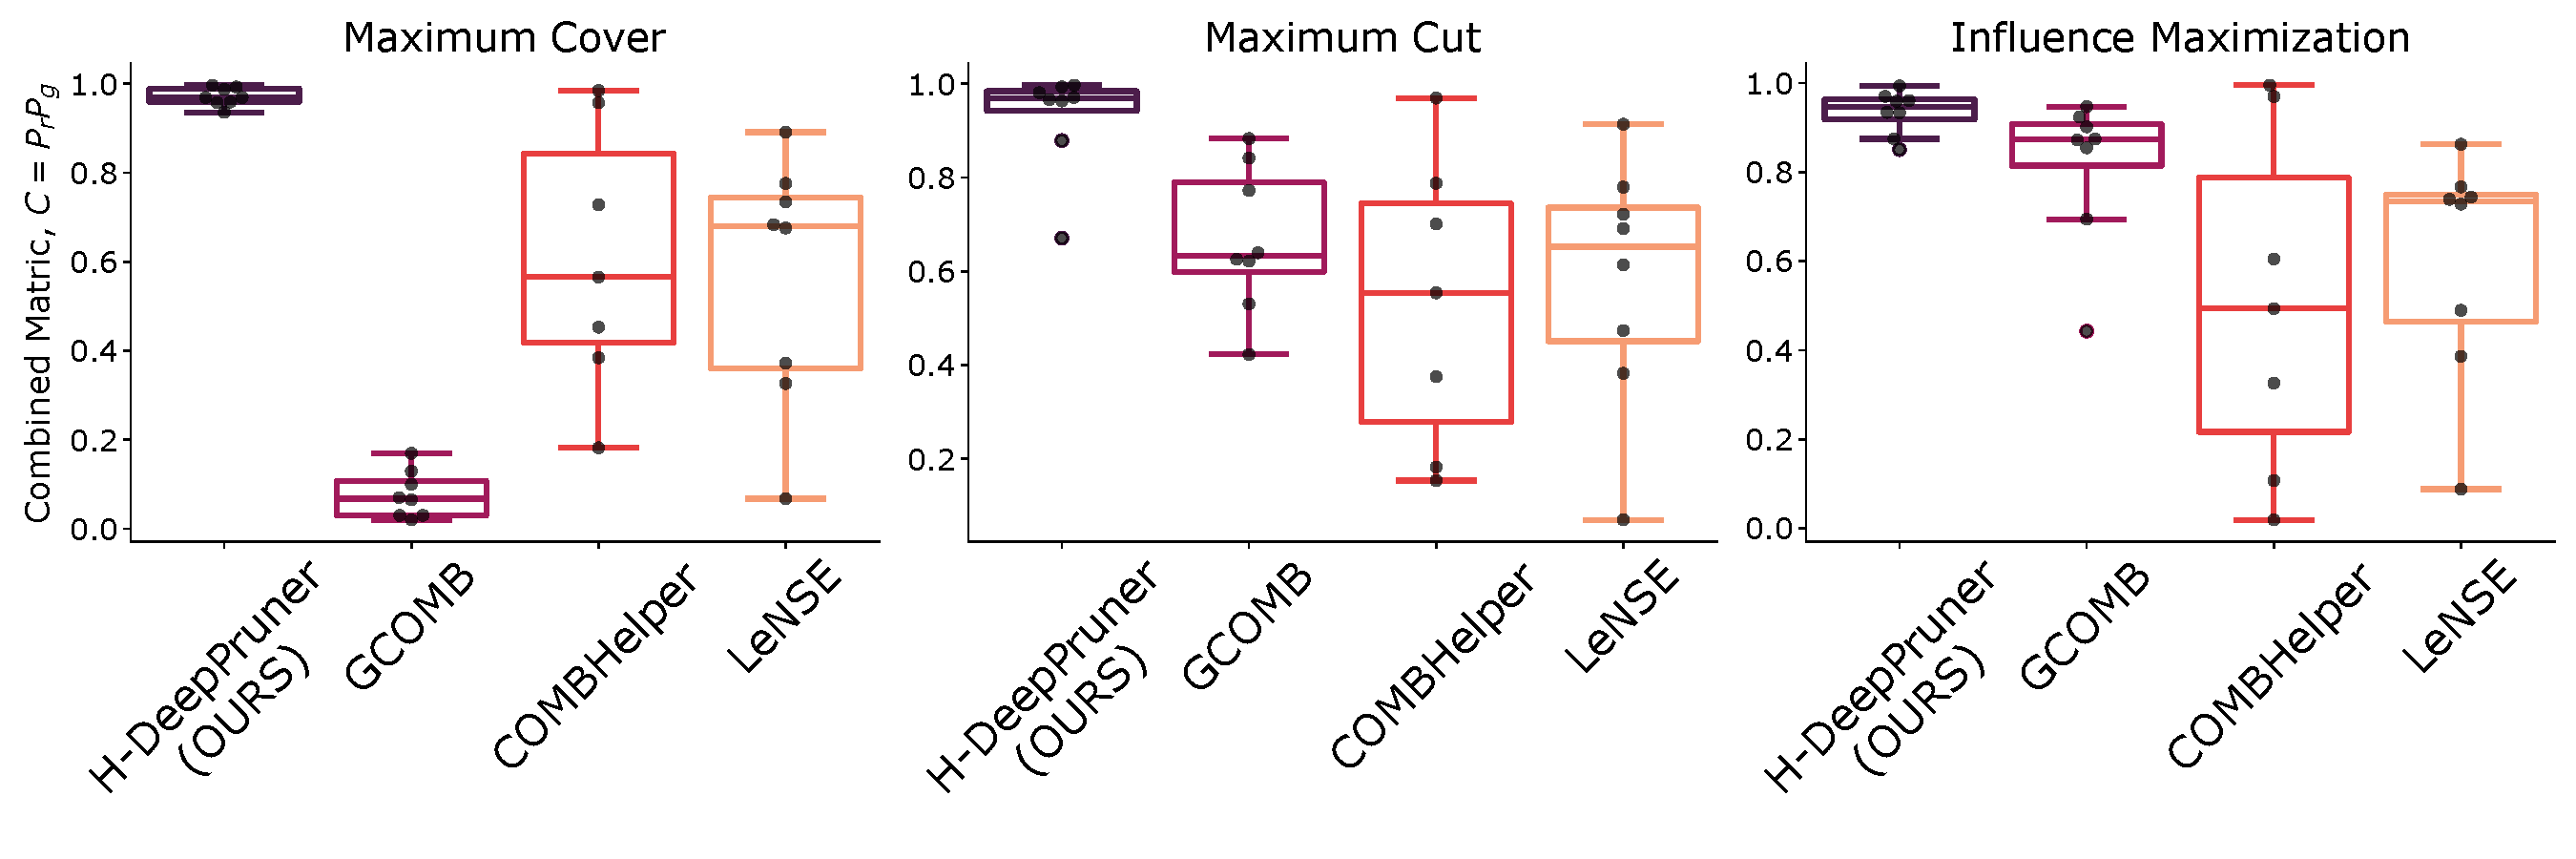
\includegraphics[width=0.9\linewidth]{violin_plots_inkspace.pdf}
    \caption{Box plots of the combined metric (higher is better) for all algorithms across all problems.}
    \label{fig:violin}
\end{figure*}

Hence, we introduce a general adaptive framework that combines supervised learning and reinforcement learning, requiring no domain-specific knowledge or feature engineering. Our proposed algorithm, Hierarchical DeepPruner (H-DeepPruner), is a two-stage pruner. In the first stage, we use a Graph Neural Network to prune the search space based on the local neighborhood of nodes. In the second stage, we prune the search space further using GNN-guided Monte Carlo Tree Search.

\paragraph{Contributions.} The contributions are summarized as follows:

\begin{itemize}
    \item  We propose an adaptive, problem-agnostic hierarchical framework for reducing the search space in CO problems on graphs, named Hierarchical DeepPruner. This framework combines supervised and reinforcement learning to accelerate heuristics that do not scale well to large problem instances. To the best of our knowledge, our algorithm is the first approach that does not require problem-specific feature engineering for pruning.

    \item We have conducted extensive experiments and compared our algorithm with three state-of-the-art pruning algorithms to demonstrate the effectiveness of our algorithm. As shown by the experimental results, our algorithm can achieve substantial reductions in ground set size (typically over 95\%) while nearly preserving the objective value across multiple budgets.

    \item Additionally, we show that all training can be done on small, random graphs while still being able to scale up to out-of-distribution larger test graphs at inference time. 
\end{itemize}

\paragraph{Organization.} The rest of this paper is organized as follows. First, we describe the relationship between our contribution and existing work and introduce preliminaries and notation. Then, we present our algorithm, H-DeepPruner, and conduct an empirical evaluation, comparing it to existing learned heuristics for the pruning problem. Finally, we conclude the paper and discuss future directions.




\section{Related Work}

\begin{figure*}[t]
    \centering
    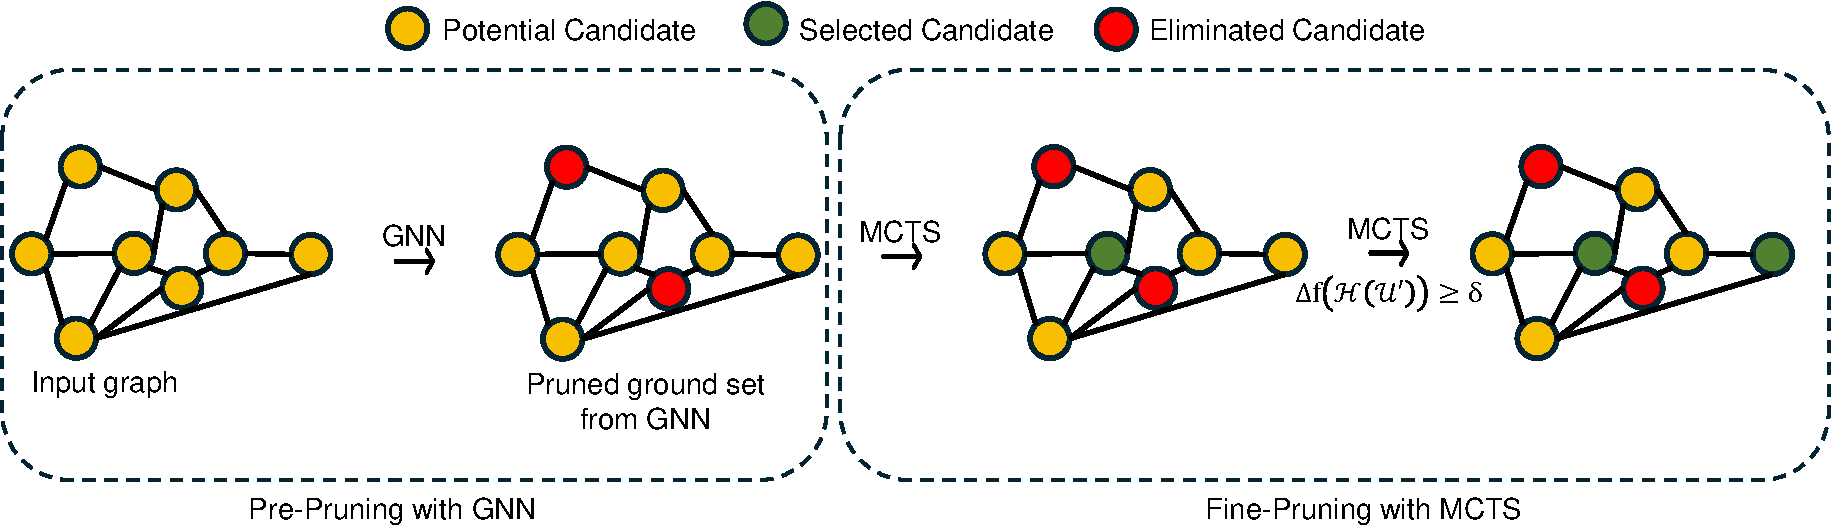
\includegraphics[width=0.95\linewidth]{H_deeppruner_cropped.pdf}
    \caption{Illustration of the proposed framework as applied to an instance. The process begins with a GNN discarding many elements that are unlikely to contribute to an optimal solution. Next, MCTS iteratively constructs a much smaller ground set with progressive deepening.}
    \label{fig:H_deeppruner}
\end{figure*}


The literature regarding reducing the search space and tree search algorithms for CO problems is vast, so we only discuss learning-based algorithms in this section as these works are the most pertinent to our algorithm.

\paragraph{Pruning Search Space for CO Problems.} To improve the scalability of heuristics, several works have proposed to prune the search space of CO problems and focus only on the reduced search space. These approaches primarily fall into two categories: supervised learning and a combination of reinforcement and supervised learning. Our approach belongs to the latter category. In a purely supervised learning setting, the general approach involves training a binary classifier to predict whether a vertex or edge in a graph can be safely removed without compromising the solution quality produced by the heuristic. These classifiers are trained using labels generated from solving instances within the training distribution. For instance, \citet{lauri2019fine} use logistic regression with hand-crafted features to prune vertices from graphs for the Maximum Clique Enumeration problem. Similarly, \citet{grassia2019learning,lauri2023learning} propose a multi-stage pruning strategy, where each stage involves training a new classifier with hand-crafted features that integrate graph-theoretic and statistical attributes. \citet{fitzpatrick2021learning,sun2021generalization} train classifiers to prune edges unlikely to belong to the optimal tour in Traveling Salesman Problem instances.


Although these methods leverage relatively simple machine learning frameworks, a major limitation is their lack of problem-agnostic design, requiring substantial problem-specific research and trial-and-error on the part of algorithm designers, making them difficult to adapt to other problems. To address this limitation, \citet{tian2024combhelper} propose COMBHelper, a GNN-based framework with knowledge distillation and a problem-specific boosting module designed to generalize to multiple CO problems on graphs. While effective across various CO problems, it relies on computationally expensive Fourier Feature Mapping and a problem-specific boosting mechanism for strong performance. This problem-specific module leverages domain knowledge to enhance results—for example, in Minimum Vertex Cover, it penalizes the model more during training when it fails to identify high-degree nodes.


Approaches that integrate supervised and reinforcement learning tend to be more problem-agnostic. For instance, GCOMB \cite{manchanda2020gcomb} uses a probabilistic greedy algorithm for training data generation and then trains a linear regression model to generate a pruned ground set using a weighted degree heuristic. A Q-learning network is then trained on the pruned search space to sequentially predict the solution. \textcolor{black}{However, a key limitation of this approach is that the initial pruning relies on a handcrafted degree heuristic, which does not generalize well to multiple CO problems (see Table \ref{tab:main} for details).} Similarly, LeNSE \citep{ireland2022lense} employs a two-stage learning process: first, a GNN is trained using supervised learning to generate graph embeddings for subgraphs sampled from graphs in the training distribution. Then, a policy network is trained to use these embeddings to guide a local search procedure, navigating from an initial subgraph to a pruned subgraph that is more likely to contain the optimal solution. A major drawback of this method is its reliance on domain expertise to categorize subgraphs into different classes, determine the number of samples per class, and tune critical hyperparameters—such as the size of the vertex subset used to induce subgraphs and the dimensionality of vertex embeddings—individually for each dataset and problem to achieve strong performance.

We compare our algorithm with three state-of-the-art (SOTA) pruning methods: GCOMB, COMBHelper, and LeNSE. We demonstrate that our algorithm typically prunes over 95\% of the ground set, as shown in Table \ref{tab:main}. It also outperforms all other methods in terms of the highest mean combined metric (defined below) across all problems, as shown in Figure \ref{fig:violin}. Additionally, unlike these approaches, which often require domain-specific knowledge and feature engineering, our method is notably simpler. This simplicity is a key strength, as it is easily generalizable to multiple CO problems. Hence, our approach is robust across different distributions and problem settings, making it applicable to a wide range of CO problems without requiring extensive modifications.


\paragraph{Tree Search Algorithms for CO problems.} One of the earliest attempts to apply deep learning to CO problems in combination with tree search is made by \citet{li2018combinatorial}, who combine a Graph Convolutional Network (GCN) \cite{kipf2016semi} with guided tree search in a supervised setting, requiring a large number of pre-solved instances for training. Similarly, \citet{abe2019solving} train a GCN using Monte Carlo Tree Search as a policy improvement operator, inspired by the AlphaGo Zero approach \cite{silver2017mastering}. \citet{xing2020graph} introduce a GNN-assisted Monte Carlo Tree Search method to construct the optimal solution to the TSP by adding nodes successively. \citet{choo2022simulation} propose a fixed-width tree search algorithm guided by a neural network-learned policy. However, the primary focus of these works is on obtaining solutions as close to optimal as possible, and these approaches are limited to graphs containing only hundreds or thousands of nodes. In contrast, our approach is orthogonal, as it accelerates heuristics by pruning the ground set rather than directly optimizing the objective function, enabling scalability to large instances.


\section{Preliminaries}

This section introduces the concept and notations used in this work. For completeness, we provide the mechanism of Graph Neural Network, Monte Carlo Tree Search and Markov Decision Process for understanding our algorithm.


\paragraph{Graph Neural Network (GNN).} A Graph Neural Network (GNN) is a type of neural network designed to learn representations of graph-structured data by iteratively aggregating and transforming information from neighboring nodes and edges. Assume we have an undirected graph $G (V, E)$ where $V$ is the set of vertices (nodes) and $E$ is the set of edges. 
Let \( N(v_i) \) be the set of neighbors of node \( v_i \), defined as \( N(v_i) \equiv \{ v_j \in V \mid A_{i,j} \neq 0 \} \), where \( A \) is the adjacency matrix of the graph $G (V, E)$.
% Let $N\left(v_i\right) \equiv \left\{v_j \in \mathcal{V}:\mathcal{A}_{i,j}\neq 0\right\}$ denote the set of neighbors of node $v_i$. 
	We construct a $k$-layer GNN as follows:
	\begin{equation*}
		\begin{aligned}
			& h_{v_i}^{\left(k\right)} \equiv  f^{\left(k\right)}_{2}\left(\left\{h_{v_i}^{\left(k-1\right)},\;f^{\left(k\right)}_{1}\left(\left\{h_{u}^{\left(k-1\right)}:u \in N\left(v_i\right)\right\}\right)\right\}\right),\\
		\end{aligned}
	\end{equation*}
	where function $f^{\left(k\right)}_1$ aggregates the feature information over the set of neighboring nodes and function $f^{\left(k\right)}_2$ combines the nodes’ hidden features from iteration $\left(k-1\right)$ with the aggregated neighborhood features, and $h_{v_i}^{\left(k-1\right)}$ denotes the hidden state of node $v_i$ in the $\left(k-1\right)^{th}$ layer. 
    Initially, $h_{v_i}^{\left(0\right)}$ is the output of an embedding function $g\left(\cdot\right)$ or raw node features.

% \subsection{Neural Monte Carlo Tree Search}

\paragraph{Neural Monte Carlo Tree Search (NMCTS).} Monte Carlo Tree Search (MCTS) is a decision-making algorithm widely used in games and complex decision processes. It operates by building a search tree and simulating outcomes to estimate the value of actions. Neural Monte Carlo Tree Search (NMCTS) integrates neural networks into MCTS to efficiently explore and evaluate large decision spaces. MCTS operates in four phases: \textbf{selection}, based
on a strategy to maximize the potential, \textbf{expansion}, where new nodes are added, \textbf{simulation}, to foresee possible outcomes and \textbf{backpropagation}, updating the node values based on simulation
results.

\noindent In the \textbf{selection} phase, the algorithm starts at the root node and successively selects a child node until reaching one that is either terminal or unexpanded. The child node is selected based on specific strategies e.g., the Predictor + Upper Confidence Bound (PUCT) formula, which incorporates the output of a neural policy network. The PUCT formula is given as:

\[PUCT = Q(s,a) + c_{puct} \cdot P(s,a) \cdot \frac{\sqrt{\sum_b N(s,b)}}{1+N(s,a)} \]

\noindent where, \(Q(s, a)\) is the average reward for taking action \(a\) in the state \(s\), \(P(s, a)\) is the prior probability of selecting action \(a\) as predicted by the policy network, \(N(s, a)\) is the visit count for the state-action pair, \(\sum_{b} N(s, b)\) is the total visit count of all actions at state \(s\), and \(c_{puct}\) is a hyperparameter that controls the balance between exploration and exploitation.  

\noindent In the \textbf{expansion} phase, upon reaching a leaf node, unless it represents a terminal state, the algorithm adds a new child node by expanding the action with the highest prior probability as predicted by the policy network. In the \textbf{simulation} phase, the newly expanded node is evaluated. If the node is terminal, the true reward is returned. Otherwise, the algorithm uses a value network to predict the expected reward from the state. Finally, in the \textbf{backpropagation} phase, the simulation outcome is propagated up the tree to update the statistics of all visited nodes, refining the estimates for future decisions.



	
% Repeatedly iterating through these stages, NMCTS incrementally constructs a decision tree, refining
% strategies for optimal decision-making in scenarios where direct calculation of the best strategy is
% infeasible due to the vastness of the state space.



\subsection{Markov Decision Process}

% The process of incrementally adding an element to a pruned ground set, starting from an empty set, is delegated to an agent that
% follows an optimal policy. To learn such a policy, we consider the traditional Markov Decision Process (MDP) setting \cite{bellman1957markovian}

We reduce the pruning process to a Markov Decision Process (MDP) \cite{bellman1957markovian}. A deterministic MDP is defined as $(\mathcal{S},\mathcal{A},\mathcal{T},\mathcal{R})$ where $\mathcal{S}$ is a set of states, $\mathcal{A}$ is a set of actions
from the state $s \in \mathcal{S}$, $T: \mathcal{S} \times \mathcal{A} \rightarrow S$ is a deterministic state transition function, and $ \mathcal{R} : \mathcal{S} \times \mathcal{A} \to  \mathbb{R}$ is an immediate reward function. In our formulation, the state $s$ represents the instance, the pruned ground set created so far, and the potential candidates for addition to the pruned ground set. An action involves adding an element to the pruned ground set, and the transition function updates the state with the newly expanded ground set. The process continues until a terminal state is reached, which occurs when a fixed number of elements have been added to the ground set (a hyperparameter in our experiments). The reward is defined as the objective value of the solution obtained from the heuristic applied to the pruned ground set.


\section{Methodology}
\begin{figure*}[t]
    \centering
    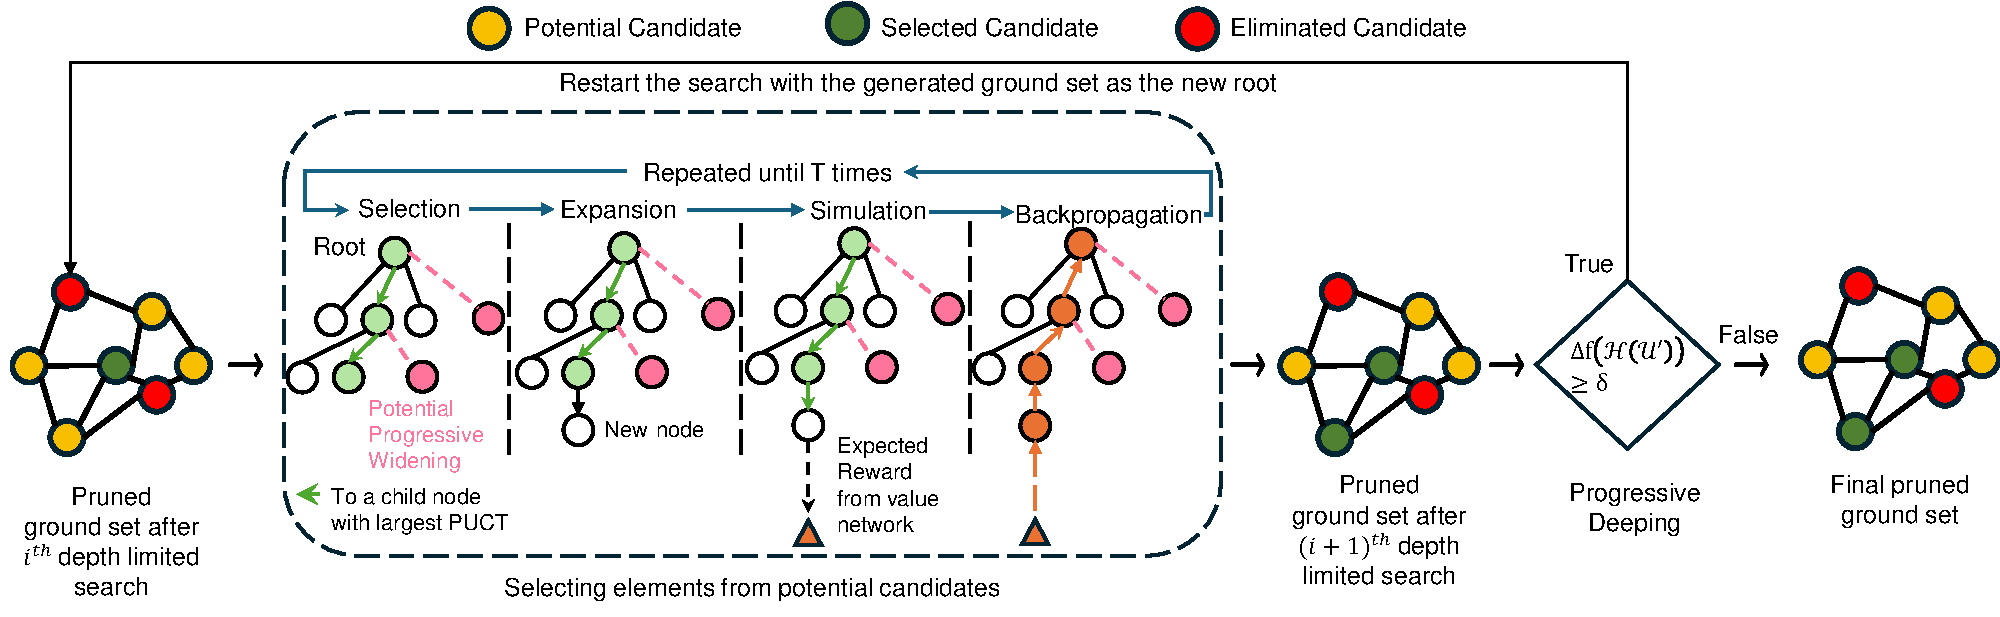
\includegraphics[width=0.9\linewidth]{MCTS_cropped.pdf}
    \caption{An illustration of MCTS with fixed depth and progressive widening for generating a pruned ground set. The search begins with an empty ground set and incrementally adds candidate elements. After each depth-limited search, a heuristic evaluates the updated pruned ground set to determine whether the solution, obtained by running the heuristic on the updated set, results in a sufficient improvement in the objective value. If successful, the search restarts with the updated ground set as the new root; otherwise, the process terminates.}
    \label{fig:MCTS}
\end{figure*}

Our proposed algorithm is schematically illustrated in Figure \ref{fig:H_deeppruner}. It consists of two main stages: an initial pruning step using a GNN, followed by NMCTS for further reduction. First, the GNN prunes the ground set in a single step, selecting elements independently of each other. Then, NMCTS refines this pruned ground set from GNN by constructing a much smaller subset from scratch while considering dependencies among elements. The following sections provide a detailed explanation of each stage.



\paragraph{Pre-Pruning with GNN.} We introduce a GNN to eliminate nodes that are unlikely to be part of the solution set, allowing NMCTS to focus computational resources on promising nodes. This step parallels the handcrafted degree heuristic in GCOMB. \textcolor{black}{ Instead of relying on a manually designed heuristic for initial pruning, we hypothesize that vertices in the optimal solution exhibit similar local structures within the graph. Therefore, they can be identified based purely on the local neighborhood of nodes rather than problem-specific features. To capture this, we adopt random node initialization \cite{abboud2020surprising}, where raw node features are set as \( h_{v_i} \sim U(0,1) \), with \( U(0,1) \) representing a uniform distribution over \([0,1]\), instead of using problem-specific features like COMBHelper and LeNSE.}

To generate training data, we use Erd{\H{o}}s-R{\'e}nyi  \citep{erdos1960evolution} (ER) graphs with $2000$ vertices and an edge probability of 
\( p = 0.1 \). We solve these graphs with a budget of $100$ using a heuristic to obtain the optimal ground set. This process produces labeled data, which we use to train the GNN in a supervised manner with weighted cross-entropy loss. \textcolor{black}{This loss prevents the non-solution vertices from dominating the training. Specifically, we use GCN as our choice of GNN. We find that many different GNN architectures can be used successfully. In general, what matters is that the network can capture relevant information about the local neighborhood of a vertex. However, we empirically observe that GNN architectures such as GraphSAGE, which uniformly sample a fixed-size set of neighbors instead of utilizing the full neighborhood, perform poorly. While this increases the computational burden of our algorithm, it remains reasonable since the initial pruning is done only once, and we use a lightweight GCN with just two layers.}

During testing, we simply discard vertices that the GNN predicts are unlikely to be in the solution set in a single pass. This approach significantly accelerates the pruning process, as the GNN can remove a large number of elements from the original ground set without compromising the objective value, as shown in Table \ref{tab:ablation}.
  
\begin{table*}[h]
\centering

\resizebox{\textwidth}{!}{%
\begin{tabular}{|ccccccccccccc|}
\hline
 &
  \multicolumn{3}{|c|}{ H-DeepPruner \textbf{(Ours})} &
  \multicolumn{3}{c|}{GCOMB*} &
  \multicolumn{3}{c|}{COMBHelper} &
  \multicolumn{3}{c|}{LeNSE*} \\ \hline
\multicolumn{1}{|c|}{Graph} &
  $P_r \uparrow$ &
  $P_g$ $\uparrow$ &
  \multicolumn{1}{c|}{$C \uparrow$} &
  $P_r \uparrow$ &
  $P_g$ $\uparrow$ &
  \multicolumn{1}{c|}{$C \uparrow$} &
  $P_r \uparrow$ &
  $P_g$ $\uparrow$ &
  \multicolumn{1}{c|}{$C \uparrow$} &
  $P_r \uparrow$ &
  $P_g$ $\uparrow$ &
  \multicolumn{1}{c|}{$C \uparrow$} \\ \hline



& \multicolumn{12}{c|}{\textbf{Maximum Cover}} \\ \hline

\multicolumn{1}{|c||}{Facebook}& 0.9849& 0.9500& \multicolumn{1}{c||}{\textbf{0.9357}}& 0.9270& 0.0700& \multicolumn{1}{c||}{0.0649}& 1.0000& 0.3840& \multicolumn{1}{c||}{0.3840}& 0.9660& 0.0700& \multicolumn{1}{c|}{0.0676}\\
\multicolumn{1}{|c||}{Wiki}& 0.9969& 0.9607& \multicolumn{1}{c||}{\textbf{0.9577}}& 0.9900& 0.0300& \multicolumn{1}{c||}{0.0297}& 1.0000& 0.4528& \multicolumn{1}{c||}{0.4528}& 1.0940& 0.3400& \multicolumn{1}{c|}{0.3720}\\
\multicolumn{1}{|c||}{Deezer}& 0.9972& 0.9953& \multicolumn{1}{c||}{\textbf{0.9925}}& 0.9940& 0.1300& \multicolumn{1}{c||}{0.1292}& 1.0000& 0.7278& \multicolumn{1}{c||}{0.7278}& 0.9790& 0.7500& \multicolumn{1}{c|}{0.7343}\\
\multicolumn{1}{|c||}{Slashdot}& 0.9900& 0.9970& \multicolumn{1}{c||}{\textbf{0.9871}}& 1.0000& 0.0200& \multicolumn{1}{c||}{0.0200}& 1.0000& 0.9844& \multicolumn{1}{c||}{0.9844}& 0.9790& 0.6900& \multicolumn{1}{c|}{0.6755}\\
\multicolumn{1}{|c||}{Twitter}& 0.9717& 0.9969& \multicolumn{1}{c||}{\textbf{0.9687}}& 0.9970& 0.1700& \multicolumn{1}{c||}{0.1695}& 1.0000& 0.5654& \multicolumn{1}{c||}{0.5654}& 0.9890& 0.3300& \multicolumn{1}{c|}{0.3264}\\
\multicolumn{1}{|c||}{DBLP}& 0.9694& 0.9994& \multicolumn{1}{c||}{\textbf{0.9688}}& 0.9990& 0.0300& \multicolumn{1}{c||}{0.0300}& 1.0000& 0.1818& \multicolumn{1}{c||}{0.1818}& 0.9900& 0.9000& \multicolumn{1}{c|}{0.8910}\\
\multicolumn{1}{|c||}{YouTube}& 0.9966& 0.9998& \multicolumn{1}{c||}{\textbf{0.9965}}& 0.9980& 0.0700& \multicolumn{1}{c||}{0.0699}& 1.0000& 0.9572& \multicolumn{1}{c||}{0.9572}& 0.9820& 0.7900& \multicolumn{1}{c|}{0.7758}\\
\multicolumn{1}{|c||}{Skitter}& 0.9591& 0.9999& \multicolumn{1}{c||}{\textbf{0.9590}}& 0.9990& 0.1000& \multicolumn{1}{c||}{0.0999}& --& --& \multicolumn{1}{c||}{--}& 0.9760& 0.7000& \multicolumn{1}{c|}{0.6832}\\
\hline
& \multicolumn{12}{c|}{\textbf{Maximum Cut}} \\ \hline

\multicolumn{1}{|c||}{Facebook}& 0.9766& 0.9000& \multicolumn{1}{c||}{\textbf{0.8789}}& 0.8130& 0.9500& \multicolumn{1}{c||}{0.7723}& 1.0000& 0.1538& \multicolumn{1}{c||}{0.1538}& 1.0000& 0.0700& \multicolumn{1}{c|}{0.0700}\\
\multicolumn{1}{|c||}{Wiki}& 0.9977& 0.9685& \multicolumn{1}{c||}{\textbf{0.9663}}& 0.9200& 0.9600& \multicolumn{1}{c||}{0.8832}& 1.0000& 0.7011& \multicolumn{1}{c||}{0.7011}& 0.9810& 0.3900& \multicolumn{1}{c|}{0.3826}\\
\multicolumn{1}{|c||}{Deezer}& 0.9979& 0.9953& \multicolumn{1}{c||}{\textbf{0.9932}}& 0.8500& 0.9900& \multicolumn{1}{c||}{0.8415}& 1.0000& 0.3754& \multicolumn{1}{c||}{0.3754}& 0.9750& 0.7400& \multicolumn{1}{c|}{0.7215}\\
\multicolumn{1}{|c||}{Slashdot}& 0.9999& 0.9970& \multicolumn{1}{c||}{\textbf{0.9970}}& 0.6320& 0.9900& \multicolumn{1}{c||}{0.6257}& 0.7935& 0.9929& \multicolumn{1}{c||}{0.7879}& 0.9900& 0.6200& \multicolumn{1}{c|}{0.6138}\\
\multicolumn{1}{|c||}{Twitter}& 0.9739& 0.9969& \multicolumn{1}{c||}{\textbf{0.9708}}& 0.6280& 0.9900& \multicolumn{1}{c||}{0.6217}& 1.0000& 0.5542& \multicolumn{1}{c||}{0.5542}& 0.9870& 0.4800& \multicolumn{1}{c|}{0.4738}\\
\multicolumn{1}{|c||}{DBLP}& 0.9642& 0.9990& \multicolumn{1}{c||}{\textbf{0.9633}}& 0.6460& 0.9900& \multicolumn{1}{c||}{0.6395}& 1.0000& 0.1825& \multicolumn{1}{c||}{0.1825}& 0.9930& 0.9200& \multicolumn{1}{c|}{0.9136}\\
\multicolumn{1}{|c||}{YouTube}& 0.9813& 0.9997& \multicolumn{1}{c||}{\textbf{0.9811}}& 0.5360& 0.9900& \multicolumn{1}{c||}{0.5306}& 0.9990& 0.9705& \multicolumn{1}{c||}{0.9695}& 0.9870& 0.7900& \multicolumn{1}{c|}{0.7797}\\
\multicolumn{1}{|c||}{Skitter}& 0.9999 &  0.6707& \multicolumn{1}{c||}{0.6706}& 0.4270& 0.9900& \multicolumn{1}{c||}{0.4227}& --& --& \multicolumn{1}{c||}{--}& 0.9740& 0.7100& \multicolumn{1}{c|}{\textbf{0.6915}}\\
\hline
& \multicolumn{12}{c|}{\textbf{Influence Maximization}} \\ \hline

\multicolumn{1}{|c||}{Facebook}& 0.9326& 0.9375& \multicolumn{1}{c||}{\textbf{0.8744}}& 0.9510& 0.7300& \multicolumn{1}{c||}{0.6942}& 1.0039& 0.3248& \multicolumn{1}{c||}{0.3261}& 0.9790& 0.0900& \multicolumn{1}{c|}{0.0881}\\
\multicolumn{1}{|c||}{Wiki}& 0.9642& 0.9685& \multicolumn{1}{c||}{\textbf{0.9339}}& 0.9690& 0.9000& \multicolumn{1}{c||}{0.8721}& 0.9969& 0.6066& \multicolumn{1}{c||}{0.6047}& 0.9600& 0.5100& \multicolumn{1}{c|}{0.4896}\\
\multicolumn{1}{|c||}{Deezer}& 0.9651& 0.9953& \multicolumn{1}{c||}{\textbf{0.9606}}& 0.8050& 0.5500& \multicolumn{1}{c||}{0.4428}& 0.9837& 0.1093& \multicolumn{1}{c||}{0.1075}& 0.9720& 0.7600& \multicolumn{1}{c|}{0.7387}\\
\multicolumn{1}{|c||}{Slashdot}& 0.9971& 0.9963& \multicolumn{1}{c||}{0.9935}& 0.9660& 0.9800& \multicolumn{1}{c||}{0.9467}& 1.0076& 0.9875& \multicolumn{1}{c||}{\textbf{0.9950}}& 0.9660& 0.7700& \multicolumn{1}{c|}{0.7438}\\
\multicolumn{1}{|c||}{Twitter}& 0.9614& 0.9975& \multicolumn{1}{c||}{\textbf{0.9590}}& 0.9200& 0.9800& \multicolumn{1}{c||}{0.9016}& 0.9972& 0.4947& \multicolumn{1}{c||}{0.4933}& 0.9660& 0.4000& \multicolumn{1}{c|}{0.3864}\\
\multicolumn{1}{|c||}{DBLP}& 0.8512& 0.9990& \multicolumn{1}{c||}{0.8504}& 0.8630& 0.9900& \multicolumn{1}{c||}{0.8544}& 0.9873& 0.0194& \multicolumn{1}{c||}{0.0192}& 0.9690& 0.8900& \multicolumn{1}{c|}{\textbf{0.8624}}\\
\multicolumn{1}{|c||}{YouTube}& 0.9702& 0.9998& \multicolumn{1}{c||}{\textbf{0.9700}}& 0.9330& 0.9900& \multicolumn{1}{c||}{0.9237}& 0.9992& 0.9705& \multicolumn{1}{c||}{0.9697}& 0.9710& 0.7500& \multicolumn{1}{c|}{0.7282}\\
\multicolumn{1}{|c||}{Skitter}& 0.9331& 0.9999& \multicolumn{1}{c||}{\textbf{0.9330}}& 0.8830& 0.9900& \multicolumn{1}{c||}{0.8742}& --& --& \multicolumn{1}{c||}{--}& 0.9830& 0.7800& \multicolumn{1}{c|}{0.7667}\\
\hline





  
\end{tabular}%
}
\caption{Comparison of pruning algorithms for size constraint experiments (best-combined metric in \textbf{bold}); *Values as reported in  \cite{ireland2022lense} and ``--" denotes no reasonable result is achieved by the corresponding algorithm under the time constraint.}
\label{tab:main}
\end{table*}



\paragraph{Fine-Pruning with NMCTS.} While the GNN can prune a large number of elements from the ground set, the pruned ground set from the GNN is still many times larger than the budget, shown in Table \ref{tab:ablation}. \textcolor{black}{Notice that pruning using the GNN completely ignores the relative importance of elements in the ground set and predicts which elements will be in the pruned ground set independently of one another. For example, consider a case where the pruned ground set from the GNN is $\mathcal{U}_{\mathit{GNN}}$ , and two elements $v_1, v_2 \in \mathcal{U}_{\mathit{GNN}}$ satisfy the condition $f( \mathcal{H}(\mathcal{U}_{\mathit{GNN}} \setminus \{ v_1, v_2 \} \cup \{ v_1 \})) = f(\mathcal{H}(\mathcal{U}_{\mathit{GNN}} \setminus \{ v_1, v_2 \} \cup \{ v_2 \})) \geq f(\mathcal{H}(\mathcal{U}_{\mathit{GNN}} \setminus \{ v_1, v_2 \})$. In this scenario, we could eliminate one of the two elements. This suggests that we can further refine the pruned ground set, making it significantly smaller. To address this, we introduce a more refined pruning approach that considers the relative importance of elements when adding them to the pruned ground set. We propose to guide a NMCTS with a fixed search depth using a GNN and an adaptive search strategy (as shown in Figure \ref{fig:MCTS}), resulting in a pruned ground set of variable size.}

\textcolor{black}{NMCTS gradually constructs a solution starting from an empty set, adding one element at a time. At each step, it evaluates the current pruned ground set, considering the elements already selected and selects elements that contribute to current pruned ground set. For training, we use the same dataset we used for training the GNN.}




During testing, we notice that the NMCTS is too slow especially for large action spaces. As a result, the number of simulations becomes intractable. So we apply \textit{progressive widening} \cite{coulom2007computing,couetoux2011continuous}, which maintains a finite list of chance
nodes (or equivalently list of actions) to be searched and
incrementally adds a new child chance node $N_c$ to the list of child nodes of parent node $N_p$ based on the visitation counts. Specifically, a new child node is added every time the following is satisfied:


\[ \lfloor \text{Number of visits}(N_p)^\alpha \rfloor \geq | \text{CHILDREN} (N_p)| \]

where $\alpha \in (0,1)$ is a parameter that controls the growth rate. For all of our experiments, we set $\alpha =0.1$. This allows gradually increasing the number of choices or actions explored during the search process, starting from a narrow focus and expanding it as more information is gained. 

We also introduce, \textit{progressive deepening}, a search strategy designed to refine the search space by iteratively expanding the search tree based on improvements in the objective value. The search starts at the root node with an empty subset and explores solutions up to a fixed depth of $50$.  Initially, the objective value is zero. Following each depth-limited search, the algorithm checks if there is a significant improvement in the objective value (at least 1\%) compared to the previous search. If an improvement is found, the search restarts from the root node using the current solution,  effectively deepening the search by focusing on promising areas.  If, however, no significant improvement is observed, signifying a potential plateau, the search terminates. This method prevents the search tree from growing uncontrollably, as it focuses on expanding only when progress is made. Empirical experiments demonstrate that progressive deepening effectively prunes unnecessary elements in the search space while sacrificing little in the overall objective value, making it an efficient approach for CO problems.



\section{Experimental Studies}
\begin{figure*}[t]
    \centering
    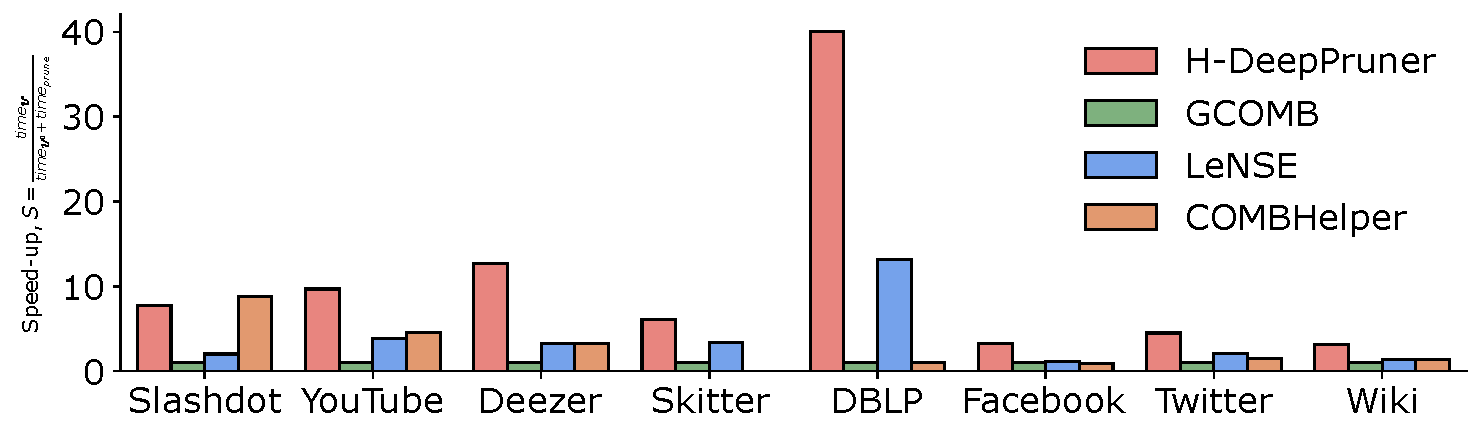
\includegraphics[width=0.85\linewidth]{speed_up_inkspace.pdf}
    \caption{The relative speed-up of using the heuristic on the pruned ground set for all algorithms across different datasets for Maximum Cover.}
    \label{fig:speedup}
\end{figure*}
In this section, we compare the empirical performance of H-DeepPruner to three SOTA pruning algorithms for 
three CO problems on graph, following the experimental setup in \citet{ireland2022lense}. We provide the code and detailed instructions for reproducing the experiments at \url{https://github.com/ankurnath/Hierarchical-DeepPruner}.

% \url{https://anonymous.4open.science/r/Hierarchical-DeepPruner-3F7C}.


\paragraph{Experimental Setup.} We run all our experiments on a Linux server equipped with an NVIDIA RTX A6000 GPU and an AMD EPYC $7713$ CPU, using PyTorch $2.4.1$ and Python $3.12.7$.

\paragraph{Applications.} We evaluate our algorithm on the following three budget-constrained problems:

\noindent \textbf{Maximum Cover (MaxCover).} Given a budget $k$ , the goal of this problem is to find a subset of nodes $S \subseteq V$ that maximizes the objective function, $f(S)= |\{v |  v \in S \lor \exists(u,v) \in E , u \in S  \}|$ where $ |S| \leq k$.

\noindent  \textbf{Maximum Cut (MaxCut).} Given a budget $k$, the goal of this problem is to find a subset of nodes $S \subseteq V$ that maximizes the objective function, $f(S)= |\{ (u,v) \in E: v \in S, u \in V \setminus S \}|$ where $ |S| \leq k$.

\noindent \textbf{Influence Maximization (IM).} Given a budget $k$, probabilities $p(u,v)$ on the edges $(u,v)\in E$ and a cascade model $\mathcal{C}$, the goal of this problem is to find a subset of nodes $S \subseteq V$ that maximizes the expected spread, $f(S)= \mathbf{E}[\sigma(S)]$ where $\sigma(S)$ denotes the spread of $S$ and $ |S| \leq k$.  For the experiments, we consider the independent cascade model \citep{kempe2003maximizing} and set $p = 0.01$ following \citet{chen2009efficient}. Because relatively large propagation probability $p$ the influence spread is not very sensitive to different algorithms and heuristics, because a giant connected component exists even after removing every edge with probability $1-p$.


In all experiments, our algorithm and the baselines are trained to create a pruned ground set for CO problems with a budget of \( k = 100 \) following \citet{ireland2022lense}. Note that the size of the pruned ground set may exceed the budget, as the heuristics will ultimately generate a solution from the ground set that adheres to the size constraint.

\paragraph{Datasets.} We evaluate our approach using real-world datasets from the Stanford Large Network Dataset Collection \citep{leskovec2016snap} for the CO problems on graphs.

\paragraph{Baselines.} We compare our approach with prior learning-based methods that have been benchmarked against classical heuristics. These methods do not directly optimize the objective function but instead accelerate heuristic solvers by pruning the ground set. We include the following baselines: GCOMB \cite{manchanda2020gcomb}, LeNSE \cite{ireland2022lense} and COMBHelper \cite{tian2024combhelper}. For training and testing the baselines, we partition the edges of the original graph into training and test sets, allocating a certain percentage for training while using the remaining edges to form the test graph. We follow the same train-test split ratio for edge sampling as described in \citet{ireland2022lense}. In contrast, our algorithm is trained on ER graphs, as described earlier.

\paragraph{Network Architecture.} The architecture for pre-pruning with GNN consists of two layers, each containing a graph convolutional layer with ReLU activation and $16$ hidden channels. The policy and value networks of NMCTS share the same backbone and use a similar architecture as the one used for pre-pruning with GNN. 


\paragraph{Evaluation Metrics.} We evaluate the algorithms using three performance metrics, where higher values indicate better performance in all cases. The first metric is the
\textit{pruning approximation ratio} $P_r$,
defined as the ratio of the objective value obtained from the pruned ground set $\mathcal{U}'$ to the objective value from the original ground set $\mathcal{U}$, both computed by a heuristic $\mathcal{H}$. Specifically, $P_r = f( \mathcal{H} (\mathcal{U}')) / f( \mathcal{H} (\mathcal{U}))$. The second metric is the
\textit{pruned fraction} $P_g$ of the original ground set that is pruned.
Finally, since an algorithm could trivially obtain the highest in one metric
by totally disregarding the other (pruning nothing or pruning everything),
we consider the \textit{combined metric}, $C = P_rP_g$. Following \citet{tian2024combhelper}, we also report \textit{speed-up}, \(  S = \frac{\text{time}_{\mathcal{U}}}{\text{time}_{\mathcal{U}'} + \text{time}_{\text{prune}}} \) where \( \text{time}_{\mathcal{U}} \) represents the running time of the heuristic on the original ground set, \( \text{time}_{\mathcal{U}'} \) is the running time of the heuristic on the pruned ground set, and \( \text{time}_{\text{prune}} \) is the time required for the pruning process.



\paragraph{Heuristics.} For MaxCover and MaxCut, we use \textsc{Standard Greedy} \cite{nemhauser1978analysis}, while for IM, we use IMM \cite{tang2015influence}.



\paragraph{Results and Analysis.} From Table \ref{tab:main}, we observe that our approach typically achieves a near-optimal pruning approximation ratio while pruning over 95\% of the original ground set. H-DeepPruner achieves the highest combined metric in 88\% of all tested instances as shown in Table \ref{tab:main}. H-DeepPruner significantly outperforms methods like COMBHelper and GCOMB, which overlook the relationships between vertices. This advantage arises because H-DeepPruner adopts a more holistic approach, taking into account the interdependencies among vertices. By considering these relationships, H-DeepPruner ensures that the selected vertices together form a well-balanced ground set, leading to better overall performance.

Notably, compared to other learning-based models, our approach does not require any computationally expensive feature computation or domain knowledge. For instance, \textsc{LeNSE} requires calculating the eigenvector centrality of each node, which is a costly calculation for large graphs. \textsc{COMBHelper} relies on a problem-specific boosting module to enhance performance. Our approach achieves a 54\% improvement in the combined metric over the leading competitor, LeNSE, with the improvement quantified as \((C_{H-Deepruner} - C_{LeNSE}) / C_{LeNSE}\).




On the other hand, the initial pruning process of GCOMB, based on a handcrafted heuristic, is computationally cheap and fast. However, except for Influence Maximization (IM), it either prunes too little (e.g., MaxCover) or too much (e.g., MaxCut), indicating that GCOMB is not problem-agnostic. Similarly, \textsc{COMBHelper} performs well in problems like Maximum Independent Set and Minimum Vertex Cover, where the pruned ground set can be large due to the absence of budget constraints, it performs poorly in problems like MaxCover and IM when the pruned ground set can be quite small without compromising performance. On the other hand, LeNSE exhibits a more balanced performance but requires tuning for each dataset and problem, whereas our approach generalizes across datasets and problems while achieving significantly greater pruning than LeNSE.











\paragraph{Multi-budget Analysis.} We investigate whether heuristics can also achieve (close-to) optimal results for budgets lower than those for which the H-DeepPruner is trained. As mentioned, in
our experiments the agent is trained to identify an optimal
subgraph for a budget of $100$. We now test whether the
subgraphs returned by H-DeepPruner can also be used to obtain an
optimal score for various budgets lower than $100$. Specifically, we report the ratio achieved when looking to find a
solution for the following budgets: $1$, $10$, $25$, $50$ and $75$ following \cite{ireland2022lense}.

Due to space constraints, we report the results for IM problem in Table \ref{tab: multi budget results}. In most cases, the ground set provided by H-DeepPruner is also the optimal ground set for budgets lower than those for which the agent is trained. For other applications, the results are qualitatively similar.
% The results for the three problems are presented in . 



\begin{table*}[h!]
              \centering
                \begin{tabular}{|c|c|c|c|c|c|c|}
                \hline
                \multirow{2}[4]{*}{\textbf{Graph}} & 
                    \multicolumn{6}{|c|}{\textbf{Budget}} \\
                    \cline{2-7} & 1 & 10 & 25 & 50 & 75 & 100 \\
                \hline
% & \multicolumn{6}{c|}{\textbf{Maximum Cover}} \\ \hline
% Facebook& 1.0000 & 1.0000 & 0.9997 & 0.9960 & 0.9900 & 0.9849 \\
% Wiki& 1.0000 & 1.0000 & 1.0000 & 1.0000 & 0.9987 & 0.9969 \\
% Deezer& 1.0000 & 1.0000 & 1.0000 & 0.9991 & 0.9996 & 0.9972 \\
% Slashdot& 1.0000 & 1.0000 & 1.0000 & 1.0000 & 0.9982 & 0.9900 \\
% Twitter& 1.0000 & 1.0000 & 1.0000 & 0.9957 & 0.9879 & 0.9717 \\
% DBLP& 1.0000 & 0.9808 & 0.9815 & 0.9775 & 0.9756 & 0.9694 \\
% YouTube& 1.0000 & 1.0000 & 1.0000 & 0.9998 & 0.9986 & 0.9966 \\
% Skitter& 1.0000 & 1.0000 & 0.9968 & 0.9851 & 0.9708 & 0.9591 \\
%  \hline
% & \multicolumn{6}{c|}{\textbf{Maximum Cut}} \\ \hline
% Facebook& 1.0000 & 1.0000 & 1.0000 & 0.9969 & 0.9879 & 0.9766 \\
% Wiki& 1.0000 & 1.0000 & 1.0000 & 1.0000 & 0.9999 & 0.9977 \\
% Deezer& 1.0000 & 1.0000 & 1.0000 & 1.0000 & 0.9997 & 0.9979 \\
% Slashdot& 1.0000 & 1.0000 & 1.0000 & 1.0000 & 1.0000 & 0.9999 \\
% Twitter& 1.0000 & 1.0000 & 1.0000 & 0.9946 & 0.9818 & 0.9739 \\
% DBLP& 1.0000 & 0.9824 & 0.9730 & 0.9704 & 0.9687 & 0.9642 \\
% YouTube& 1.0000 & 1.0000 & 1.0000 & 0.9982 & 0.9904 & 0.9813 \\
% Skitter& 1.0000 & 0.9077 & 0.7970 & 0.7543 & 0.7145 & 0.6707 \\
%  \hline
& \multicolumn{6}{c|}{\textbf{Influence Maximization}} \\ \hline
Facebook& 1.0842 & 0.9902 & 0.9782 & 0.9549 & 0.9319 & 0.9662 \\
Wiki& 1.0630 & 1.0142 & 1.0010 & 1.0214 & 0.9681 & 0.9694 \\
Deezer& 0.9476 & 0.9275 & 0.9668 & 1.0105 & 0.9853 & 0.9960 \\
Slashdot& 1.0112 & 1.0573 & 0.9609 & 0.9756 & 1.0192 & 0.9855 \\
Twitter& 1.0244 & 0.9895 & 0.9497 & 0.9763 & 0.9821 & 0.9177 \\
DBLP& 0.6147 & 0.6587 & 0.7629 & 0.8096 & 0.8517 & 0.8352 \\
YouTube& 1.0343 & 1.0045 & 1.0221 & 0.9920 & 0.9566 & 0.9583 \\
Skitter& 0.9800 & 1.0424 & 0.9620 & 0.9946 & 0.9291 & 0.9494 \\
 \hline

                \end{tabular}
                \caption{Results showing the ratio achieved for the IM problem, for budgets lower than that which the H-DeepPruner is trained to attain.}
                \label{tab: multi budget results}
            \end{table*}


% \paragraph{Scalability.}
\begin{table*}[h]
\centering


\resizebox{\textwidth}{!}{%
\begin{tabular}{@{}ccccccccccccccccccc@{}}
\toprule
                              & \multicolumn{6}{c}{Maximum Cover}                                                                                                            & \multicolumn{6}{c}{Maximum Cut}                                                                                                             & \multicolumn{6}{c}{Influence Maximization}                                                                                                  \\ \cmidrule(lr){2-7} \cmidrule(lr){8-13}  \cmidrule(lr){14-19} 
                              & \multicolumn{3}{c}{GNN}                                               & \multicolumn{3}{c}{H-DeepPruner}                         & \multicolumn{3}{c}{GNN}                                              & \multicolumn{3}{c}{H-DeepPruner}                          & \multicolumn{3}{c}{GNN}                                              & \multicolumn{3}{c}{H-DeepPruner}                          \\ \midrule
\multicolumn{1}{c|}{Graph}    & $P_r \uparrow$ & $P_g$ $\uparrow$ & \multicolumn{1}{c|}{$C \uparrow$} & $P_r \uparrow$ & $P_g$ $\uparrow$ & \multicolumn{1}{c|}{$C\uparrow$} & $P_r \uparrow$ & $P_g$ $\uparrow$ & \multicolumn{1}{c|}{$C\uparrow$} & $P_r \uparrow$ & $P_g$ $\uparrow$ & \multicolumn{1}{c|}{$C\uparrow$} & $P_r \uparrow$ & $P_g$ $\uparrow$ & \multicolumn{1}{c|}{$C\uparrow$} & $P_r \uparrow$ & $P_g$ $\uparrow$ & \multicolumn{1}{c|}{$C\uparrow$} \\ \midrule

\multicolumn{1}{c|}{Facebook}& 0.9974& 0.7789& \multicolumn{1}{c|}{0.7768}& 0.9849& 0.9500& \multicolumn{1}{c|}{0.9357}& 1.0000& 0.7651& \multicolumn{1}{c|}{0.7651}& 0.9766& 0.9000& \multicolumn{1}{c|}{0.8789}& 1.0091& 0.4555& \multicolumn{1}{c|}{0.4597}& 0.9326& 0.9375& 0.8744\\
\multicolumn{1}{c|}{Wiki}& 1.0000& 0.8633& \multicolumn{1}{c|}{0.8633}& 0.9969& 0.9607& \multicolumn{1}{c|}{0.9577}& 1.0000& 0.8643& \multicolumn{1}{c|}{0.8643}& 0.9977& 0.9685& \multicolumn{1}{c|}{0.9663}& 0.9792& 0.7660& \multicolumn{1}{c|}{0.7500}& 0.9642& 0.9685& 0.9339\\
\multicolumn{1}{c|}{Deezer}& 1.0000& 0.7625& \multicolumn{1}{c|}{0.7625}& 0.9972& 0.9953& \multicolumn{1}{c|}{0.9925}& 1.0000& 0.7539& \multicolumn{1}{c|}{0.7539}& 0.9979& 0.9953& \multicolumn{1}{c|}{0.9932}& 1.0056& 0.4111& \multicolumn{1}{c|}{0.4134}& 0.9651& 0.9953& 0.9606\\
\multicolumn{1}{c|}{Slashdot}& 1.0000& 0.8567& \multicolumn{1}{c|}{0.8567}& 0.9900& 0.9970& \multicolumn{1}{c|}{0.9871}& 1.0000& 0.8685& \multicolumn{1}{c|}{0.8685}& 0.9999& 0.9970& \multicolumn{1}{c|}{0.9970}& 0.9882& 0.7487& \multicolumn{1}{c|}{0.7398}& 0.9971& 0.9963& 0.9935\\
\multicolumn{1}{c|}{Twitter}& 1.0000& 0.8518& \multicolumn{1}{c|}{0.8518}& 0.9717& 0.9969& \multicolumn{1}{c|}{0.9687}& 1.0000& 0.8522& \multicolumn{1}{c|}{0.8522}& 0.9739& 0.9969& \multicolumn{1}{c|}{0.9708}& 1.0096& 0.6840& \multicolumn{1}{c|}{0.6906}& 0.9614& 0.9975& 0.9590\\
\multicolumn{1}{c|}{DBLP}& 1.0000& 0.7899& \multicolumn{1}{c|}{0.7899}& 0.9694& 0.9994& \multicolumn{1}{c|}{0.9688}& 1.0000& 0.7974& \multicolumn{1}{c|}{0.7974}& 0.9642& 0.9990& \multicolumn{1}{c|}{0.9633}& 1.0117& 0.5147& \multicolumn{1}{c|}{0.5208}& 0.8512& 0.9990& 0.8504\\
\multicolumn{1}{c|}{YouTube}& 1.0000& 0.8437& \multicolumn{1}{c|}{0.8437}& 0.9966& 0.9998& \multicolumn{1}{c|}{0.9965}& 1.0000& 0.8555& \multicolumn{1}{c|}{0.8555}& 0.9813& 0.9997& \multicolumn{1}{c|}{0.9811}& 0.9494& 0.6588& \multicolumn{1}{c|}{0.6255}& 0.9702& 0.9998& 0.9700\\
\multicolumn{1}{c|}{Skitter}& 1.0000& 0.8625& \multicolumn{1}{c|}{0.8625}& 0.9591& 0.9999& \multicolumn{1}{c|}{0.9590}& 1.0000& 0.6289 & \multicolumn{1}{c|}{0.6289}& 0.9999 & 0.6707 & \multicolumn{1}{c|}{0.6706}& 0.9934& 0.6053& \multicolumn{1}{c|}{0.6013}& 0.9331& 0.9999& 0.9330\\


\bottomrule
\end{tabular}%
}
\caption{H-DeepPruner, including both a GNN and NMCTS trained on the same distributions and abalations (as described in the text on the SNAP datasets for budget 100)}
\label{tab:ablation}
\end{table*}
\paragraph{Ablation Study.} The key components of H-DeepPruner are: (\romannumeral 1) a single-pass GNN pruning step to quickly discard elements from the ground set, and (\romannumeral 2) the construction of a reduced ground set using NMCTS with progressive widening and deepening.

Ablation studies of the GNN and NMCTS confirm that both are essential for strong performance as shown in Table \ref{tab:ablation}. While removing the GNN has a limited impact on the pruning approximation ratio, it significantly improves NMCTS scalability. Thus, the utility of the GNN becomes more pronounced in larger instances, where only a smaller fraction of the search space can be explored within a fixed computation budget. NMCTS, on the other hand, tries to prune the ground set from GNN further without sacrificing the pruning approximation ratio. Due to space constraints, additional ablations on generalization and progressive deepening are deferred to the full version of the paper, which will be made available on arXiv.




\paragraph{Efficiency and Scalability Study.} \textcolor{black}{Following \citet{tian2024combhelper}, we report the speed-up (as defined above) of heuristics as they optimize over a significantly smaller subset of the original ground set (as shown in Figure \ref{fig:speedup}). The results show that our approach accelerates the heuristic by up to $40$ times by effectively pruning a large portion of the ground set. This efficiency and scalability of our approach is further highlighted in Figure \ref{fig:memory}, where we observe that COMBHelper has the highest combined memory usage, making it the most computationally demanding algorithm. In contrast, H-DeepPruner follows closely behind, while LeNSE shows relatively minimal memory usage. This difference can be attributed to LeNSE's design, which modifies only a subgraph and thus does not require loading the entire graph into memory.}
\begin{figure}[t]
    \centering
    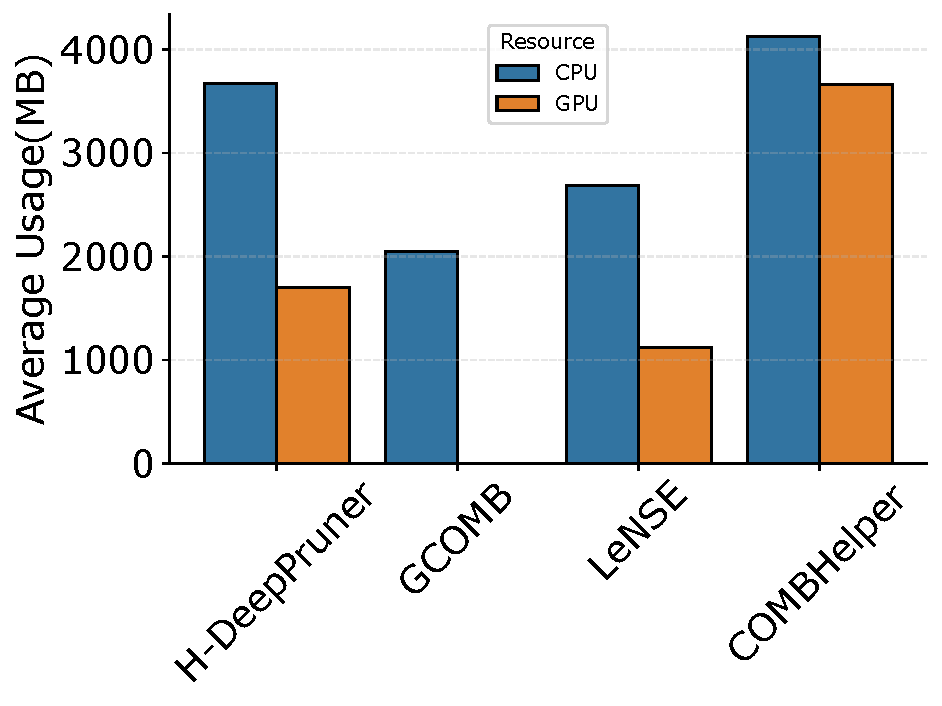
\includegraphics[width=0.8\linewidth]{cpu_gpu_usage_by_algorithm_inkspace.pdf}
    \caption{Average GPU and CPU memory utilization among algorithms for MaxCover on YouTube dataset.}
    \label{fig:memory}
\end{figure}
\section{Conclusion}
We have introduced H-DeepPruner, a novel graph pruning algorithm that identifies a reduced ground set containing the optimal solution of a CO problem. Unlike most previous methods, which are manually designed for specific CO problems, H-DeepPruner is a general framework that can be combined with any existing heuristic of choice for large-scale problems. In all the settings we have investigated using real-world graph datasets, we find that training can be done on small instances of random graphs while still scaling up to the large out-of-distribution graphs without performance degradation. Additionally, the reduced ground set found by H-DeepPruner is substantially smaller than the original ground set. Furthermore, we demonstrate that the reduced ground set identified by H-DeepPruner is, in most cases, also optimal for budgets lower than those the model is trained to recognize. We compare H-DeepPruner to three SOTA learning-based pruning approaches and find that our algorithm provides a better ratio while pruning a significantly larger portion of the ground set.


\bibliography{aaai25}

\end{document}
